\capitulo{3}{Conceptos teóricos}

En este apartado se van a explicar aquellos conceptos teóricos básicos que son necesarios para comprender el proyecto.


\section{Sistema de Información}



\subsection{Definición}

Para comenzar, hay que explicar que no existe una definición de consenso en la propia definición de Sistema de Información. De hecho, existen multitud de definiciones diferentes sobre cómo se define un Sistema de Información.


Los autores Laudon y Laudon definen un Sistema de Información como un conjunto de módulos relacionados ente sí que son capaces de obtener(o reutilizar), procesar, almacenar y distribuir cierta información para que sirva de apoyo para la toma de decisiones \cite{vicen}.
A parte de suministrar apoyo en decisiones importantes, también pueden ayudar a detectar problemas o carencias difíciles de ver sin la ayuda de estos sistemas.


\subsection{Componentes de un Sistema de Información}
Aunque existen numerosas definiciones y no existe una definición general o global, la mayoría de Sistemas de Información pueden representarse a través del diagrama de la figura \ref{fig:componentesSI}.



\imagenflotante{componentesSI}{Componentes de un Sistema de Información}

Se pueden apreciar 5 elementos principales. En primer lugar los elementos de entrada, que en nuestro proyecto serían los ficheros (.xls) originales descargados de \emph{Sigma}. 

A continuación estaría un elemento de modificación o transformación, que en nuestro caso sería el preprocesado de los ficheros originales anteriores en ficheros (.csv) reordenados, modificados y sin ningún tipo de error. También se podría incluir la carga de datos a la Base de Datos creada con anterioridad.

Seguidamente estaría el sistema de salida, donde se visualizan los resultados obtenidos. En este proyecto, el sistema de salida serían los diferentes tipos de gráficos que se pueden obtener a partir de la información que seleccione el usuario y los datos existentes o disponibles en la BBDD.

Además de estas 3 secciones, se aprecian otras dos secciones más. Una de ellas es el mecanismo de control, que es el proceso encargado de lograr los objetivos, que sería el quinto y último elemento.
En nuestro proyecto se podrían identificar numerosos mecanismos de control, como por ejemplo que los ficheros que se puedan seleccionar en los botones de \emph{Preprocesar} y \emph{Cargar Archivos} sean únicamente (.xls) y (.csv) respectivamente. Otros mecanismos de control serían la no introdución de datos repetidos en la BBDD o la selección de opciones de datos que realmente se encuentran en la BBDD, entre otros.

En cuanto a los objetivos de nuestro sistema de información, hay que destacar que se definen en el apartado anterior denominado \emph{Objetivos del proyecto}.

\subsection{Características de un Sistema de Información}



\subsection{Tipos de Sistemas de Información}



\subsection{Ventajas de un Sistema de Información}



\section{Parseado de Datos}
El Preprocesado / Parseado de ficheros es un proceso mediante el cual...





\section{Gráficos Representados}

\subsection{Diagrama de Caja y Bigotes}
Los diagramas de cajas y bigotes (o diagramas de cuartiles) son un tipo de gráficas que representan una gran cantidad de información de manera muy visual y esquematizada. A su vez, se pueden apreciar características estadísticas relevantes como la simetría y la dispersión de un conjunto de datos.

Toda esta valiosa información se representa mediante unas pequeñas cajas muy intuitivas, como se aprecia en la figura \ref{fig:caja}.

%\imagenflotante{caja}{Información de Caja y Bigotes}
	
	\begin{figure}%[!h]
		\centering
		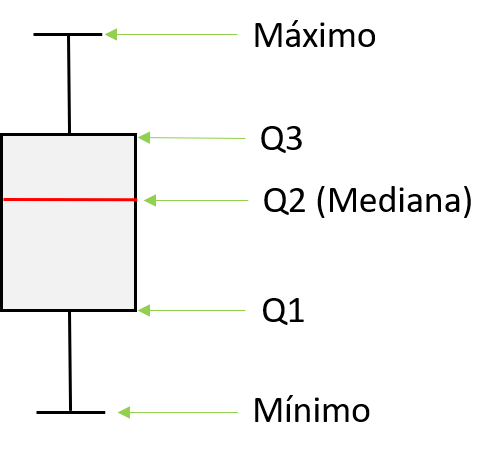
\includegraphics[width=0.6\textwidth]{caja}
		\caption{Información de Caja y Bigotes}\label{fig:caja}
	\end{figure}
	
Se diferencian cinco partes fundamentales: 
\begin{itemize}
	\item 
	\textbf{Tres Cuartiles (Q1, Q2 y Q3).} Hay que destacar que el segundo cuartil(Q2) coincide con la mediana y representa la relación entre el primer y tercer cuartil. El primer cuartil identifica el valor por debajo del cual queda un 25\% de todos los datos de la muestra ordenada. Del mismo modo, el tercer cuartil es el valor por debajo del cual quedan el 75\% de los datos de la muestra.
	\item 
	\textbf{Máximo.} Representa el valor máximo de los datos.
	\item 
	\textbf{Mínimo.} Representa el valor mínimo de los datos.
\end{itemize}

\subsection{Gráfico de Barras}
